\chapter{My Second Chapter}
\section[Short title]{Reasonably Long Section Title}

Email ID of Krishna Kumar \href{mailto:kks32@cam.ac.uk}{kks32@cam.ac.uk}. The SI Units for dynamic viscosity is \si{\newton\second\per\metre\squared}. I'm going to randomly include a picture~\cref{fig:minion}


\begin{figure}[htbp!] 
\centering    

\includegraphics[width=0.5\textwidth]{Chapter2/Figs/minion.jpg}
\caption[Minion]{This is just a long figure caption for the minion in Despicable Me from Pixar}
\label{fig:minion}
\end{figure}


\section*{Enumeration}
\begin{enumerate}
\item The first topic is dull
\item The second topic is duller
\begin{enumerate}
\item The first subtopic is silly
\item The second subtopic is stupid
\end{enumerate}
\item The third topic is dullest
\end{enumerate}

\section*{itemize}
\begin{itemize}
\item The first topic is dull
\item The second topic is duller
\begin{itemize}
\item The first subtopic is silly
\item The second subtopic is stupid
\end{itemize}
\item The third topic is dullest
\end{itemize}

\section*{description}
\begin{description}
\item[The first topic] is dull
\item[The second topic] is duller
\begin{description}
\item[The first subtopic] is silly
\item[The second subtopic] is stupid
\end{description}
\item[The third topic] is dullest
\end{description}


\clearpage

\tochide\section{Hidden Section}
\textbf{Lorem ipsum dolor sit amet}, \textit{consectetur adipiscing elit}. In magna nisi, aliquam id blandit id, congue ac est. Fusce porta consequat leo. Proin feugiat at felis vel consectetur. Ut tempus ipsum sit amet congue posuere. Nulla varius rutrum quam. Donec sed purus luctus, faucibus velit id, ultrices sapien. Cras diam purus, tincidunt eget tristique ut, egestas quis nulla. Curabitur vel iaculis lectus. Nunc nulla urna, ultrices et eleifend in, accumsan ut erat. In ut ante leo. Aenean a lacinia nisl, sit amet ullamcorper dolor. Maecenas blandit, tortor ut scelerisque congue, velit diam volutpat metus, sed vestibulum eros justo ut nulla. Etiam nec ipsum non enim luctus porta in in massa. Cras arcu urna, malesuada ut tellus ut, pellentesque mollis risus.Morbi vel tortor imperdiet arcu auctor mattis sit amet eu nisi. Nulla gravida urna vel nisl egestas varius. Aliquam posuere ante quis malesuada dignissim. Mauris ultrices tristique eros, a dignissim nisl iaculis nec. Praesent dapibus tincidunt mauris nec tempor. Curabitur et consequat nisi. Quisque viverra egestas risus, ut sodales enim blandit at. Mauris quis odio nulla. Cras euismod turpis magna, in facilisis diam congue non. Mauris faucibus nisl a orci dictum, et tempus mi cursus.

Etiam elementum tristique lacus, sit amet eleifend nibh eleifend sed \footnote{My footnote goes blah blah blah! \dots}. Maecenas dapibus augue ut urna malesuada, non tempor nibh mollis. Donec sed sem sollicitudin, convallis velit aliquam, tincidunt diam. In eu venenatis lorem. Aliquam non augue porttitor tellus faucibus porta et nec ante. Proin sodales, libero vitae commodo sodales, dolor nisi cursus magna, non tincidunt ipsum nibh eget purus. Nam rutrum tincidunt arcu, tincidunt vulputate mi sagittis id. Proin et nisi nec orci tincidunt auctor et porta elit. Praesent eu dolor ac magna cursus euismod. Integer non dictum nunc.


\begin{landscape}

\section*{Subplots}
I can cite Wall-E (see ~\cref{fig:WallE}) and Minions in despicable me (~\cref{fig:Minnion}) or I can cite the whole figure as ~\cref{fig:animations}


\begin{figure}
  \centering
  \subfloat[A Tom and Jerry]{\label{fig:TomJerry}
\includegraphics[width=0.3\textwidth]{Chapter2/Figs/TomandJerry.jpg}}                
  \subfloat[A Wall-E]{\label{fig:WallE}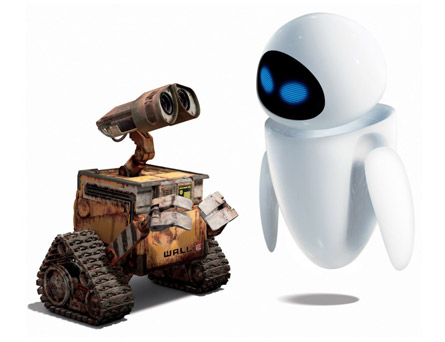
\includegraphics[width=0.3\textwidth]{Chapter2/Figs/WallE.jpg}}
  \subfloat[A Minion]{\label{fig:Minnion}
\includegraphics[width=0.3\textwidth]{Chapter2/Figs/minion.jpg}}
  \caption{Best Animations}
  \label{fig:animations}
\end{figure}


\end{landscape}
